\documentclass[11pt,a4paper]{article}
\usepackage{geometry}
\geometry{margin=1in}
\usepackage{amsmath,amssymb}
\usepackage{fontspec}
\usepackage{xcolor}
\usepackage{tikz}
\usetikzlibrary{arrows.meta, calc, angles, quotes, patterns}
\usepackage[most]{tcolorbox}

\tcbuselibrary{skins, breakable}

% Bengali Font Setup (XeLaTeX)
\setmainfont{Kalpurush}[Script=Bengali]

% Define Custom tcolorboxes
\newtcolorbox{qbox}[1]{
    enhanced,
    breakable,
    colframe=red!75!black,
    colback=red!4!white,
    coltitle=white,
    fonttitle=\bfseries\large,
    title={#1},
    arc=1.5mm,
    boxrule=1.2pt
}

\newtcolorbox{solbox}{
    enhanced,
    breakable,
    colframe=blue!75!black,
    colback=blue!4!white,
    coltitle=white,
    fonttitle=\bfseries\large,
    title={সমাধান},
    arc=1.5mm,
    boxrule=1.2pt
}

\title{\textbf{ভেক্টর ক্যালকুলাস ও গতিবিদ্যা: গাণিতিক সমস্যা ও সমাধান}}
\author{Vector Calculus \& Dynamics Problems}
\date{}

\begin{document}

\maketitle

% ---------------------------------------------------------
% QUESTION 11
% ---------------------------------------------------------
\begin{qbox}{প্রশ্ন ১১}
\textbf{প্রশ্ন:} যদি $\phi(x,y,z) = xy^2z$ এবং $\vec{A} = xz\hat{i} - xy^2\hat{j} + yz^2\hat{k}$ হয়, তবে ত্রিমাত্রিক ভেক্টর ক্যালকুলাসের আংশিক অন্তরীকরণ ব্যবহার করে $(2, -1, 1)$ বিন্দুতে $\frac{\partial^3(\phi \vec{A})}{\partial x^2 \partial z}$ এর মান নির্ণয় করো। \\
\textit{(\textbf{English:} If $\phi(x,y,z) = xy^2z$ and $\vec{A} = xz\hat{i} - xy^2\hat{j} + yz^2\hat{k}$, then using partial differentiation of 3D vector calculus, find the value of $\frac{\partial^3(\phi \vec{A})}{\partial x^2 \partial z}$ at the point $(2, -1, 1)$.)}
\end{qbox}

\begin{solbox}
প্রথমে স্কেলার ক্ষেত্র $\phi$ এবং ভেক্টর ক্ষেত্র $\vec{A}$ এর গুণফল নির্ণয় করি:
$$\phi \vec{A} = (xy^2z)(xz\hat{i} - xy^2\hat{j} + yz^2\hat{k})$$
$$\Rightarrow \phi \vec{A} = x^2y^2z^2\hat{i} - x^2y^4z\hat{j} + xy^3z^3\hat{k}$$

এখন, $x$ এর সাপেক্ষে প্রথমবার আংশিক অন্তরীকরণ (partial differentiation) করি:
$$\frac{\partial(\phi \vec{A})}{\partial x} = \frac{\partial}{\partial x}(x^2y^2z^2\hat{i} - x^2y^4z\hat{j} + xy^3z^3\hat{k})$$
$$\Rightarrow \frac{\partial(\phi \vec{A})}{\partial x} = 2xy^2z^2\hat{i} - 2xy^4z\hat{j} + y^3z^3\hat{k}$$

এবার $x$ এর সাপেক্ষে দ্বিতীয়বার আংশিক অন্তরীকরণ করি:
$$\frac{\partial^2(\phi \vec{A})}{\partial x^2} = \frac{\partial}{\partial x}(2xy^2z^2\hat{i} - 2xy^4z\hat{j} + y^3z^3\hat{k})$$
$$\Rightarrow \frac{\partial^2(\phi \vec{A})}{\partial x^2} = 2y^2z^2\hat{i} - 2y^4z\hat{j}$$

অবশেষে, প্রাপ্ত মানটিকে $z$ এর সাপেক্ষে আংশিক অন্তরীকরণ করি:
$$\frac{\partial^3(\phi \vec{A})}{\partial x^2 \partial z} = \frac{\partial}{\partial z}(2y^2z^2\hat{i} - 2y^4z\hat{j})$$
$$\Rightarrow \frac{\partial^3(\phi \vec{A})}{\partial x^2 \partial z} = 4y^2z\hat{i} - 2y^4\hat{j}$$

এখন $(2, -1, 1)$ বিন্দুতে অর্থাৎ $x = 2$, $y = -1$ এবং $z = 1$ বসিয়ে পাই:
$$\frac{\partial^3(\phi \vec{A})}{\partial x^2 \partial z} = 4(-1)^2(1)\hat{i} - 2(-1)^4\hat{j} = 4\hat{i} - 2\hat{j}$$

\textbf{উত্তর:} $4\hat{i} - 2\hat{j}$
\end{solbox}

\vspace{0.4cm}

% ---------------------------------------------------------
% QUESTION 12
% ---------------------------------------------------------
\begin{qbox}{প্রশ্ন ১২}
\textbf{প্রশ্ন:} একটি স্রোতস্বিনী নদীতে এমনভাবে নৌকা চালনা করা হলো যেন নৌকাটি ন্যূনতম পথে (সরাসরি প্রস্থ বরাবর) অপর তীরে পৌঁছায়। এতে যে সময় লাগে, নদীতে কোনো স্রোত না থাকলে সরাসরি প্রস্থ বরাবর পার হতে তার অর্ধেক সময় লাগত। নৌকার নিজস্ব বেগ $2\text{ m/s}$ হলে স্রোতের বেগ নির্ণয় করো। \\
\textit{(\textbf{English:} A boat is steered across a river such that it reaches the opposite bank along the shortest path (straight across the width). The time taken for this is twice the time it would take to cross directly across the width if there were no current. If the boat's own speed is $2\text{ m/s}$, find the velocity of the river current.)}
\end{qbox}

\begin{solbox}
\begin{center}
\begin{tikzpicture}[scale=0.85, >=Stealth]
    % River banks
    \draw[thick, fill=blue!10] (-1,0) rectangle (7,3);
    \draw[ultra thick, blue!80!black] (-1,0) -- (7,0);
    \draw[ultra thick, blue!80!black] (-1,3) -- (7,3);
    
    % Nodes & Coordinates
    \coordinate (A) at (2,0);
    \coordinate (B) at (2,3);
    \coordinate (C) at (0.2,0);
    
    % Vectors
    \draw[->, very thick, red] (A) -- (C) node[midway, above] {স্রোতের বেগ $\vec{u}$};
    \draw[->, very thick, green!50!black] (A) -- (B) node[midway, left] {লব্ধি বেগ $\vec{w} = \sqrt{v^2-u^2}$};
    \draw[->, very thick, blue] (A) -- ($(B)+(A)-(C)$) node[midway, above right] {নৌকার বেগ $\vec{v}$};
    \draw[dashed] (B) -- ($(B)+(A)-(C)$);
    
    % Annotations
    \node[below=3pt] at (A) {আদি স্থান ($P$)};
    \node[above] at (B) {সোজা বিপরীত পাড়};
    \draw[<->] (6,0) -- (6,3) node[midway, right] {প্রস্থ $d$};
\end{tikzpicture}
\end{center}

ধরি, নদীর প্রস্থ = $d$, নৌকার বেগ = $v = 2\text{ m/s}$ এবং স্রোতের বেগ = $u$।

১. \textbf{ন্যূনতম বা সোজাসুজি পথে নদী পারাপারের ক্ষেত্রে:} \\
সোজাসুজি নদী পার হতে লব্ধি বেগের দিক স্রোতের সাথে $90^\circ$ হতে হবে। এই ক্ষেত্রে লব্ধি বেগ $w = \sqrt{v^2 - u^2}$।

অতএব, ন্যূনতম পথে নদী পার হতে প্রয়োজনীয় সময়:
$$t = \frac{d}{w} = \frac{d}{\sqrt{v^2 - u^2}} \quad \text{--- (i)}$$

২. \textbf{স্রোত না থাকলে সোজাসুজি পারাপারের ক্ষেত্রে:} \\
স্রোত না থাকলে নৌকাটি সরাসরি $v$ বেগে অপর পাড়ে যাবে। প্রয়োজনীয় সময়:
$$t' = \frac{d}{v} \quad \text{--- (ii)}$$

শর্তানুসারে, স্রোতযুক্ত ন্যূনতম পথের সময় স্রোতবিহীন সময়ের দ্বিগুণ ($t = 2t'$ বা $t' = \frac{1}{2}t$):
$$\frac{d}{v} = \frac{d}{2\sqrt{v^2 - u^2}}$$

উভয় পক্ষ থেকে $d$ বাদ দিয়ে এবং বর্গ করে পাই:
$$\frac{1}{v^2} = \frac{1}{4(v^2 - u^2)}$$
$$\Rightarrow 4v^2 - 4u^2 = v^2$$
$$\Rightarrow 3v^2 = 4u^2 \implies u = \frac{\sqrt{3}}{2}v$$

দেওয়া আছে, নৌকার বেগ $v = 2\text{ m/s}$। মানটি বসিয়ে পাই:
$$u = \frac{\sqrt{3}}{2} \times 2 = \sqrt{3}\text{ m/s} \approx 1.732\text{ m/s}$$

\textbf{উত্তর:} $\sqrt{3}\text{ m/s}$ (বা $1.732\text{ m/s}$)
\end{solbox;

\vspace{0.4cm}

% ---------------------------------------------------------
% QUESTION 13
% ---------------------------------------------------------
\begin{qbox}{প্রশ্ন ১৩}
\textbf{প্রশ্ন:} একটি বিমান $500\text{ km/h}$ গতিতে উত্তর দিকে অনুভূমিকভাবে উড়ে যাচ্ছে। বিমানের এক যাত্রী একটি বিশেষ বন্দুক দিয়ে সোজা উপরের দিকে (উল্লম্বভাবে) $1000\text{ km/h}$ আপেক্ষিক বেগে একটি গুলি ছুড়ল। মাটিতে দাঁড়িয়ে থাকা একজন স্থির পর্যবেক্ষকের সাপেক্ষে গুলিটির লব্ধি বেগ কত হবে এবং এটি উল্লম্বের সাথে কত কোণ উৎপন্ন করবে? \\
\textit{(\textbf{English:} An airplane is flying horizontally northward at a speed of $500\text{ km/h}$. A passenger on the plane fires a bullet straight upwards (vertically) with a relative speed of $1000\text{ km/h}$ using a special gun. With respect to a stationary observer on the ground, what will be the resultant velocity of the bullet and what angle will it make with the vertical?)}
\end{qbox}

\begin{solbox}
\begin{center}
\begin{tikzpicture}[scale=0.95, >=Stealth]
    % Axes
    \draw[->, thick, gray] (-0.5,0) -- (3.5,0) node[right] {উত্তর ($\hat{i}$)};
    \draw[->, thick, gray] (0,-0.5) -- (0,4.5) node[above] {উল্লম্ব ($\hat{j}$)};
    
    % Coordinates
    \coordinate (O) at (0,0);
    \coordinate (V) at (0,3.6);
    \coordinate (P) at (1.8,3.6);
    
    % Vectors
    \draw[->, ultra thick, blue] (O) -- (1.8,0) node[midway, below] {$\vec{v}_p = 500\hat{i}$};
    \draw[->, ultra thick, red] (1.8,0) -- (P) node[midway, right] {$\vec{v}_{g/p} = 1000\hat{j}$};
    \draw[->, ultra thick, purple] (O) -- (P) node[midway, above left] {$\vec{v}_g$};
    
    \draw[dashed] (V) -- (P);
    \draw[dashed] (O) -- (V);
    
    % Angle arc
    \pic [draw, angle radius=0.8cm, "$\theta$", angle eccentricity=1.3] {angle = P--O--V};
\end{tikzpicture}
\end{center}

ধরি, উত্তর দিক বরাবর অনুভূমিক একক ভেক্টর $\hat{i}$ এবং খাড়া উপরের দিক বরাবর উল্লম্ব একক ভেক্টর $\hat{j}$।

মাটির সাপেক্ষে বিমানের বেগ, $\vec{v}_p = 500\hat{i}\text{ km/h}$

বিমানের সাপেক্ষে গুলির আপেক্ষিক বেগ, $\vec{v}_{g/p} = 1000\hat{j}\text{ km/h}$

ভেক্টর যোগের আপেক্ষিক সূত্রানুসারে, মাটির সাপেক্ষে গুলির প্রকৃত বেগ ($\vec{v}_g$):
$$\vec{v}_g = \vec{v}_p + \vec{v}_{g/p} = (500\hat{i} + 1000\hat{j})\text{ km/h}$$

গুলির লব্ধি বেগের মান:
$$|\vec{v}_g| = \sqrt{500^2 + 1000^2} = \sqrt{250000 + 1000000} = \sqrt{1250000} \approx 1118.03\text{ km/h}$$

\textbf{উল্লম্বের সাথে উৎপন্ন কোণ ($\theta$):}

গুলির বেগ ভেক্টরটি উল্লম্ব অক্ষ ($\hat{j}$) এর সাথে $\theta$ কোণ তৈরি করলে:
$$\tan\theta = \frac{v_x}{v_y} = \frac{500}{1000} = 0.5$$
$$\Rightarrow \theta = \tan^{-1}(0.5) \approx 26.565^\circ$$

\textbf{উত্তর:} লব্ধি বেগ $1118.03\text{ km/h}$ এবং উল্লম্বের সাথে কোণ $26.565^\circ$
\end{solbox}

\vspace{0.4cm}

% ---------------------------------------------------------
% QUESTION 14
% ---------------------------------------------------------
\begin{qbox}{প্রশ্ন ১৪}
\textbf{প্রশ্ন:} $2\text{ m/s}$ বেগে বয়ে যাওয়া অনুভূমিক বাতাসের অভিমুখে একটি গাড়ি $12\text{ m/s}$ বেগে চলছে। গাড়িটির সামনের উইন্ডশিল্ডের কোণ $\angle A = 35^\circ$ এবং পিছনের কাচের কোণ $\angle B = 60^\circ$ (উভয় কোণ অনুভূমিকের সাথে)। গাড়িটি চলার সময় সামনের কাচে বৃষ্টি খাড়া লম্বভাবে পড়ছে। \\
(ক) বৃষ্টির প্রকৃত বেগ নির্ণয় করো। \\
(খ) বৃষ্টি কি গাড়িটির পিছনের কাচে সরাসরি আঘাত করবে? গাণিতিকভাবে বিশ্লেষণ করো। \\
\textit{(\textbf{English:} A car moves at $12\text{ m/s}$ in the direction of a horizontal wind blowing at $2\text{ m/s}$. The angle of the front windshield is $\angle A = 35^\circ$ and the rear glass angle is $\angle B = 60^\circ$ (both with respect to the horizontal). While moving, rain falls perpendicularly on the front windshield. (a) Determine the actual velocity of the rain. (b) Will the rain hit the rear glass directly? Analyze mathematically.)}
\end{qbox}

\begin{solbox}
\begin{center}
\begin{tikzpicture}[scale=0.85]
    % Road
    \draw[thick] (-1,0) -- (9,0);
    
    % Car schematic
    \draw[ultra thick, black] (1,0) -- (1,1) -- (2.5,1) -- (4,2.5) -- (6,2.5) -- (7.5,1) -- (8.5,1) -- (8.5,0);
    
    % Windshields
    \draw[line width=1.5mm, blue] (2.5,1) -- (4,2.5) node[midway, above left] {$\angle A = 35^\circ$};
    \draw[line width=1.5mm, red] (6,2.5) -- (7.5,1) node[midway, above right] {$\angle B = 60^\circ$};
    
    % Rain relative vector
    \draw[->, ultra thick, teal] (2,3.5) -- (3.25,1.75) node[midway, left] {আপেক্ষিক বৃষ্টি};
    \draw[dashed] (3.25,1.75) -- (2.5,1);
    
    % Angles representation
    \draw (2.5,1) -- (4,1);
    \draw (3,1) arc (0:45:0.5);
    \node at (3.3,1.3) {$35^\circ$};
    
    \draw (7.5,1) -- (6,1);
    \draw (7,1) arc (180:135:0.5);
    \node at (6.7,1.3) {$60^\circ$};
\end{tikzpicture}
\end{center}

\textbf{(ক) বৃষ্টির প্রকৃত বেগ নির্ণয়:}

গাড়ি ও বাতাস একই অভিমুখে গতিশীল। গাড়ির সাপেক্ষে বাতাসের আপেক্ষিক অনুভূমিক বেগ:
$$v_{rel, x} = v_{wind} - v_{car} = 2 - 12 = -10\text{ m/s}$$

ধরি, বৃষ্টির প্রকৃত খাড়া নিচের দিকের বেগ = $V_r$।

গাড়ির সাপেক্ষে বৃষ্টির আপেক্ষিক বেগ অনুভূমিকের সাথে $35^\circ$ কোণ উৎপন্ন করে (যেহেতু এটি $35^\circ$ কোণে থাকা সামনের কাচে লম্বভাবে আপতিত হয়):
$$\tan 35^\circ = \frac{\text{Horizontal relative velocity}}{\text{Vertical velocity}} = \frac{10}{V_r}$$
$$\Rightarrow V_r = \frac{10}{\tan 35^\circ} \approx 14.28\text{ m/s}$$

অতএব, বৃষ্টির প্রকৃত বেগ খাড়া নিচের দিকে $14.28\text{ m/s}$।

\textbf{(খ) পিছনের কাচে বৃষ্টি আঘাত করবে কি না তার বিশ্লেষণ:}

গাড়ির সাপেক্ষে বৃষ্টির আপেক্ষিক গতিপথ অনুভূমিকের সাথে $35^\circ$ কোণ তৈরি করে। অর্থাৎ, উল্লম্বের সাথে এই কোণটি হলো:
$$\theta = 90^\circ - 35^\circ = 55^\circ$$

পিছনের কাচটি অনুভূমিকের সাথে $60^\circ$ কোণে হেলে আছে, যার উল্লম্বের সাথে কোণ $90^\circ - 60^\circ = 30^\circ$।

পিছনের কাচে বৃষ্টি সরাসরি না আঘাত করার জন্য আপেক্ষিক বৃষ্টির কোণ উল্লম্বের সাথে $30^\circ$ এর বেশি হতে হবে।

যেহেতু আপেক্ষিক বৃষ্টির উল্লম্ব কোণ $55^\circ > 30^\circ$, সেহেতু বৃষ্টির ফোটা সরাসরি পিছনের কাচে আঘাত করবে না।

\textbf{উত্তর:} (ক) $14.28\text{ m/s}$; (খ) পিছনের কাচে সরাসরি আঘাত করবে না।
\end{solbox}

\vspace{0.4cm}

% ---------------------------------------------------------
% QUESTION 15
% ---------------------------------------------------------
\begin{qbox}{প্রশ্ন ১৫}
\textbf{প্রশ্ন:} $r = 45\text{ cm}$ ব্যাসার্ধ বিশিষ্ট একটি চাকা অনুভূমিক রাস্তায় না পিছলিয়ে বিশুদ্ধ ঘূর্ণন গতিতে গড়াচ্ছে (pure rolling)। চাকার পরিধির উপর অবস্থিত সর্বনিম্ন স্পর্শবিন্দু $P$ যদি চাকাটির সিকি ঘূর্ণন (quarter rotation বা $90^\circ$ ঘূর্ণন) সম্পন্ন করে, তবে $P$ বিন্দুর নিট সরণ ভেক্টরের মান কত হবে? \\
\textit{(\textbf{English:} A wheel of radius $r = 45\text{ cm}$ rolls on a horizontal road in pure rolling motion without slipping. If the lowest point of contact $P$ on the circumference undergoes a quarter rotation ($90^\circ$ turn), what will be the magnitude of the net displacement vector of point $P$?)}
\end{qbox}

\begin{solbox}
\begin{center}
\begin{tikzpicture}[scale=0.95, >=Stealth]
    % Ground
    \draw[thick] (-0.5,0) -- (6.5,0);
    \fill[pattern=north east lines] (-0.5,-0.2) rectangle (6.5,0);
    
    % Initial position
    \draw[thick, fill=gray!10] (1.5,1.5) circle (1.5);
    \fill[red] (1.5,0) circle (2.5pt) node[below] {$P(0,0)$};
    \draw[dashed] (1.5,1.5) -- (1.5,0);
    
    % Final position after 90 deg
    \draw[thick, fill=gray!10] (4.5,1.5) circle (1.5);
    \fill[blue] (6.0,1.5) circle (2.5pt) node[right] {$P'(x,y)$};
    \draw[dashed] (4.5,1.5) -- (6.0,1.5);
    \draw[dashed] (4.5,1.5) -- (4.5,0);
    
    % Net Displacement Arrow
    \draw[->, ultra thick, purple] (1.5,0) -- (6.0,1.5) node[midway, above left] {সরণ $\vec{s}$};
    
    % Distance indicators
    \draw[<->] (1.5,-0.5) -- (4.5,-0.5) node[midway, below] {$x_c = r\frac{\pi}{2}$};
\end{tikzpicture}
\end{center}

চাকাটি পিছলে না গিয়ে বিশুদ্ধ ঘূর্ণন করায়, $90^\circ$ ($\theta = \frac{\pi}{2}\text{ rad}$) ঘূর্ণনের জন্য চাকার কেন্দ্রের অনুভূমিক সরণ হবে:
$$x_c = r\theta = r\left(\frac{\pi}{2}\right)$$

আদি স্পর্শবিন্দুকে মূলবিন্দু $(0,0)$ ধরলে, $90^\circ$ ঘূর্ণন শেষে $P$ বিন্দুর নতুন স্থানাঙ্ক:

অনুভূমিক সরণ ($x$):
$$x = x_c + r\sin(90^\circ) = r\frac{\pi}{2} + r = r\left(\frac{\pi}{2} + 1\right)$$

উল্লম্ব সরণ ($y$):
$$y = r - r\cos(90^\circ) = r(1 - 0) = r$$

নিট সরণ ভেক্টরের মান ($s$):
$$s = \sqrt{x^2 + y^2} = \sqrt{\left[r\left(\frac{\pi}{2} + 1\right)\right]^2 + r^2} = r\sqrt{\left(\frac{\pi}{2} + 1\right)^2 + 1^2}$$
$$s = r\sqrt{\frac{\pi^2}{4} + \pi + 1 + 1} = r\sqrt{\frac{\pi^2}{4} + \pi + 2}$$

এখানে $r = 45\text{ cm} = 0.45\text{ m}$ বসিয়ে পাই:
$$s = 0.45 \times \sqrt{\frac{3.1416^2}{4} + 3.1416 + 2} \approx 0.45 \times \sqrt{2.4674 + 3.1416 + 2}$$
$$s \approx 0.45 \times \sqrt{7.609} \approx 0.45 \times 2.758 \approx 1.241\text{ m}$$

\textbf{উত্তর:} $1.241\text{ m}$ (বা $124.1\text{ cm}$)
\end{solbox}

\vspace{0.4cm}

% ---------------------------------------------------------
% QUESTION 16
% ---------------------------------------------------------
\begin{qbox}{প্রশ্ন ১৬}
\textbf{প্রশ্ন:} ত্রিমাত্রিক বলবিদ্যায় একটি কণার অবস্থান ভেক্টর $\vec{A}(t)$ এর মান যদি সময়ের সাথে পরিবর্তিত না হয়ে সর্বদা ধ্রুবক থাকে (অর্থাৎ $|\vec{A}| = \text{constant}$), তবে ডট গুণফলের অন্তরীকরণ সূত্র ব্যবহার করে প্রমাণ করো যে, কণাটির ব্যবকলনীয় ভেক্টর $\frac{d\vec{A}}{dt}$ সর্বদা মূল ভেক্টর $\vec{A}$ এর উপর লম্ব হবে। \\
\textit{(\textbf{English:} In 3D mechanics, if the magnitude of the position vector $\vec{A}(t)$ of a particle remains constant over time (i.e., $|\vec{A}| = \text{constant}$), prove using the derivative rule for dot products that the derivative vector $\frac{d\vec{A}}{dt}$ is always perpendicular to the original vector $\vec{A}$.)}
\end{qbox}

\begin{solbox}
যেহেতু ভেক্টর $\vec{A}$ এর মান ধ্রুবক, তাই:
$$|\vec{A}| = A = \text{constant}$$

আমরা জানি, যেকোনো ভেক্টরের নিজের সাথে ডট গুণফল তার মানের বর্গের সমান:
$$\vec{A} \cdot \vec{A} = |\vec{A}|^2 = A^2 = \text{constant}$$

উভয় পক্ষকে সময়ের সাপেক্ষে অন্তরীকরণ করি:
$$\frac{d}{dt}(\vec{A} \cdot \vec{A}) = \frac{d}{dt}(A^2)$$

ডট গুণফলের অন্তরীকরণের গুণন সূত্র প্রয়োগ করে পাই:
$$\frac{d\vec{A}}{dt} \cdot \vec{A} + \vec{A} \cdot \frac{d\vec{A}}{dt} = 0$$

যেহেতু ডট গুণফল বিনিময় নিয়ম মেনে চলে ($\frac{d\vec{A}}{dt} \cdot \vec{A} = \vec{A} \cdot \frac{d\vec{A}}{dt}$):
$$2\left(\vec{A} \cdot \frac{d\vec{A}}{dt}\right) = 0 \implies \vec{A} \cdot \frac{d\vec{A}}{dt} = 0$$

যেহেতু দুটি অশূন্য ভেক্টরের ডট গুণফল শূন্য, সেহেতু ভেক্টরদ্বয় পরস্পরের উপর লম্ব।

অতএব, $\frac{d\vec{A}}{dt}$ ভেক্টরটি সর্বদা $\vec{A}$ এর উপর লম্ব। \hfill \textit{(প্রমাণিত)}
\end{solbox}

\vspace{0.4cm}

% ---------------------------------------------------------
% QUESTION 17
% ---------------------------------------------------------
\begin{qbox}{প্রশ্ন ১৭}
\textbf{প্রশ্ন:} দুটি ভেক্টর $\vec{A}$ এবং $\vec{B}$ এর লব্ধি $\vec{R}$ শুধুমাত্র y-অক্ষ বরাবর কাজ করে এবং এর মান $8\text{ unit}$। যদি $\vec{A}$ ভেক্টরটি x-অক্ষের ধনাত্মক দিকে অবস্থিত একটি একক ভেক্টরের $8$ গুণ হয়, তবে ভেক্টর বীজগণিত ব্যবহার করে $\vec{B}$ ভেক্টরের মান ও x-অক্ষের ধনাত্মক দিকের সাথে উৎপন্ন কোণ নির্ণয় করো। \\
\textit{(\textbf{English:} The resultant $\vec{R}$ of two vectors $\vec{A}$ and $\vec{B}$ acts solely along the y-axis with a magnitude of $8\text{ unit}$. If vector $\vec{A}$ is $8$ times a unit vector pointing in the positive x-direction, determine the magnitude of vector $\vec{B}$ and the angle it forms with the positive x-axis using vector algebra.)}
\end{qbox}

\begin{solbox}
\begin{center}
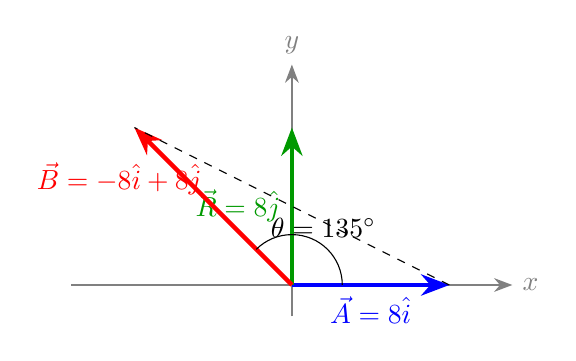
\begin{tikzpicture}[scale=0.8, >=Stealth]
    % Cartesian plane
    \draw[->, gray, thick] (-3.5,0) -- (3.5,0) node[right] {$x$};
    \draw[->, gray, thick] (0,-0.5) -- (0,3.5) node[above] {$y$};
    
    % Vectors
    \draw[->, ultra thick, blue] (0,0) -- (2.5,0) node[midway, below] {$\vec{A} = 8\hat{i}$};
    \draw[->, ultra thick, green!60!black] (0,0) -- (0,2.5) node[midway, left] {$\vec{R} = 8\hat{j}$};
    \draw[->, ultra thick, red] (0,0) -- (-2.5,2.5) node[midway, above left] {$\vec{B} = -8\hat{i} + 8\hat{j}$};
    
    % Dashed lines completing triangle
    \draw[dashed] (2.5,0) -- (-2.5,2.5);
    
    % Angle arc
    \draw (0.8,0) arc (0:135:0.8);
    \node at (0.5,0.9) {$\theta = 135^\circ$};
\end{tikzpicture}
\end{center}

প্রশ্নমতে, $\vec{A}$ ভেক্টরটি x-অক্ষ বরাবর এবং এর মান $8$:
$$\vec{A} = 8\hat{i}$$

লব্ধি ভেক্টর $\vec{R}$ শুধুমাত্র y-অক্ষ বরাবর এবং এর মান $8$:
$$\vec{R} = 8\hat{j}$$

লব্ধি ভেক্টরের সমীকরণ হতে:
$$\vec{R} = \vec{A} + \vec{B} \implies \vec{B} = \vec{R} - \vec{A}$$
$$\vec{B} = 8\hat{j} - 8\hat{i} = -8\hat{i} + 8\hat{j}$$

$\vec{B}$ ভেক্টরের মান:
$$|\vec{B}| = \sqrt{(-8)^2 + 8^2} = \sqrt{64 + 64} = \sqrt{128} = 8\sqrt{2}\text{ unit} \approx 11.31\text{ unit}$$

\textbf{x-অক্ষের ধনাত্মক দিকের সাথে উৎপন্ন কোণ ($\theta$):}

এখানে $B_x < 0$ এবং $B_y > 0$, ফলে ভেক্টরটি দ্বিতীয় চতুর্ভাগে (second quadrant) অবস্থিত:
$$\theta = 180^\circ - \tan^{-1}\left(\frac{|B_y|}{|B_x|}\right) = 180^\circ - \tan^{-1}\left(\frac{8}{8}\right)$$
$$\theta = 180^\circ - 45^\circ = 135^\circ$$

\textbf{উত্তর:} মান $8\sqrt{2}\text{ unit}$ এবং কোণ $135^\circ$
\end{solbox}

\vspace{0.4cm}

% ---------------------------------------------------------
% QUESTION 18
% ---------------------------------------------------------
\begin{qbox}{প্রশ্ন ১৮}
\textbf{প্রশ্ন:} $\vec{a} = 2\hat{i} + 3\hat{j} - \hat{k}$ এবং $\vec{b} = \hat{j} + \hat{k}$ দুটি ভেক্টর। অপর একটি ভেক্টর $\vec{c}$ প্রথম ভেক্টরদ্বয়ের সাথে সমতলীয় (coplanar)। যদি $\vec{c}$ ভেক্টরটি $\vec{a}$ এর উপর লম্ব এবং $\vec{c} \cdot \vec{b} = 24$ হয়, তবে ভেক্টর $\vec{c}$ এবং এর মান নির্ণয় করো। \\
\textit{(\textbf{English:} Two vectors are given as $\vec{a} = 2\hat{i} + 3\hat{j} - \hat{k}$ and $\vec{b} = \hat{j} + \hat{k}$. Another vector $\vec{c}$ is coplanar with the first two vectors. If vector $\vec{c}$ is perpendicular to $\vec{a}$ and $\vec{c} \cdot \vec{b} = 24$, find the vector $\vec{c}$ and its magnitude.)}
\end{qbox}

\begin{solbox}
ধরি, $\vec{c} = x\hat{i} + y\hat{j} + z\hat{k}$।

১. \textbf{সমতলীয় (coplanar) হওয়ার শর্তানুসারে:} \\
ভেক্টর তিনটি সমতলীয় হওয়ায় এদের স্কেলার ত্রয়ী গুণফল শূন্য হবে:
$$\begin{vmatrix} x & y & z \\ 2 & 3 & -1 \\ 0 & 1 & 1 \end{vmatrix} = 0$$
$$\Rightarrow x(3 - (-1)) - y(2 - 0) + z(2 - 0) = 0$$
$$\Rightarrow 4x - 2y + 2z = 0 \implies 2x - y + z = 0 \quad \text{--- (i)}$$

২. \textbf{$\vec{c} \perp \vec{a}$ হওয়ার শর্তানুসারে:}
$$\vec{c} \cdot \vec{a} = 0 \implies 2x + 3y - z = 0 \quad \text{--- (ii)}$$

৩. \textbf{দেওয়া আছে $\vec{c} \cdot \vec{b} = 24$:}
$$(x\hat{i} + y\hat{j} + z\hat{k}) \cdot (0\hat{i} + \hat{j} + \hat{k}) = 24 \implies y + z = 24 \quad \text{--- (iii)}$$

সমীকরণ (i) এবং (ii) যোগ করে পাই:
$$(2x - y + z) + (2x + 3y - z) = 0 \implies 4x + 2y = 0 \implies y = -2x \quad \text{--- (iv)}$$

সমীকরণ (iv) কে (iii)-এ বসিয়ে পাই:
$$-2x + z = 24 \implies z = 24 + 2x \quad \text{--- (v)}$$

$y$ ও $z$ এর মান (i)-এ বসিয়ে পাই:
$$2x - (-2x) + (24 + 2x) = 0 \implies 6x + 24 = 0 \implies x = -4$$

$x$ এর মান থেকে পাই:
$$y = -2(-4) = 8, \quad z = 24 + 2(-4) = 16$$

অতএব, ভেক্টরটি $\vec{c} = -4\hat{i} + 8\hat{j} + 16\hat{k}$।

$\vec{c}$ ভেক্টরের মান:
$$|\vec{c}| = \sqrt{(-4)^2 + 8^2 + 16^2} = \sqrt{16 + 64 + 256} = \sqrt{336} = 4\sqrt{21} \approx 18.33\text{ unit}$$

\textbf{উত্তর:} $\vec{c} = -4\hat{i} + 8\hat{j} + 16\hat{k}$ এবং মান $4\sqrt{21}$
\end{solbox}

\vspace{0.4cm}

% ---------------------------------------------------------
% QUESTION 19
% ---------------------------------------------------------
\begin{qbox}{প্রশ্ন ১৯}
\textbf{প্রশ্ন:} একটি গতিশীল কণার অবস্থান স্থানাঙ্কসমূহ $x = 2t^2$, $y = t^2 - 4t$ এবং $z = 3t - 5$ সমীকরণ দ্বারা নির্দেশিত হয়। $t = 1\text{ s}$ সময়ে $\vec{b} = \hat{i} - 3\hat{j} + 2\hat{k}$ ভেক্টরের অভিমুখে কণাটির ত্বরণের উপাংশ (component of acceleration) এর মান নির্ণয় করো। \\
\textit{(\textbf{English:} The position coordinates of a moving particle are given by the equations $x = 2t^2$, $y = t^2 - 4t$, and $z = 3t - 5$. At time $t = 1\text{ s}$, calculate the magnitude of the component of the particle's acceleration along the direction of the vector $\vec{b} = \hat{i} - 3\hat{j} + 2\hat{k}$.)}
\end{qbox}

\begin{solbox}
কণাটির অবস্থান ভেক্টর $\vec{r}$:
$$\vec{r} = 2t^2\hat{i} + (t^2 - 4t)\hat{j} + (3t - 5)\hat{k}$$

তাৎক্ষণিক বেগ, $\vec{v} = \frac{d\vec{r}}{dt}$:
$$\vec{v} = 4t\hat{i} + (2t - 4)\hat{j} + 3\hat{k}$$

তাৎক্ষণিক ত্বরণ, $\vec{a} = \frac{d\vec{v}}{dt}$:
$$\vec{a} = 4\hat{i} + 2\hat{j}$$

ত্বরণ ভেক্টরটি সময়-স্বাধীন (constant acceleration), তাই $t = 1\text{ s}$ সময়েও $\vec{a} = 4\hat{i} + 2\hat{j}$।

এখন, $\vec{b} = \hat{i} - 3\hat{j} + 2\hat{k}$ ভেক্টরের অভিমুখে ত্বরণের উপাংশ ($a_b$):
$$a_b = \frac{\vec{a} \cdot \vec{b}}{|\vec{b}|} = \frac{(4\hat{i} + 2\hat{j}) \cdot (\hat{i} - 3\hat{j} + 2\hat{k})}{\sqrt{1^2 + (-3)^2 + 2^2}}$$
$$a_b = \frac{4(1) + 2(-3) + 0(2)}{\sqrt{1 + 9 + 4}} = \frac{4 - 6}{\sqrt{14}} = -\frac{2}{\sqrt{14}}\text{ unit}$$

উপাংশের পরম মান (magnitude):
$$|a_b| = \frac{2}{\sqrt{14}}\text{ unit} \approx 0.535\text{ unit}$$

\textbf{উত্তর:} $\frac{2}{\sqrt{14}}$ (বা $0.535$)
\end{solbox}

\vspace{0.4cm}

% ---------------------------------------------------------
% QUESTION 20
% ---------------------------------------------------------
\begin{qbox}{প্রশ্ন ২০}
\textbf{প্রশ্ন:} যদি একটি ত্রিমাত্রিক স্কেলার ক্ষেত্র $f(x,y,z) = xy^2 + 2y^2z + z^3x$ হয়, তবে ভেক্টর ডিফারেন্সিয়াল অপারেটর (ডেল/ন্যাবলা) ব্যবহার করে $(1,1,1)$ বিন্দুতে ডাইভারজেন্স অব গ্রেডিয়েন্ট অর্থাৎ ল্যাপলাসিয়ান $\vec{\nabla}\cdot(\vec{\nabla}f)$ এর মান নির্ণয় করো। \\
\textit{(\textbf{English:} If a 3D scalar field is $f(x,y,z) = xy^2 + 2y^2z + z^3x$, use the vector differential operator (del/nabla) to find the value of the divergence of the gradient, i.e., the Laplacian $\vec{\nabla}\cdot(\vec{\nabla}f)$, at the point $(1,1,1)$.)}
\end{qbox}

\begin{solbox}
স্কেলার ক্ষেত্রের গ্রেডিয়েন্টের ডাইভারজেন্স হলো ল্যাপলাসিয়ান অপারেটর:
$$\vec{\nabla}\cdot(\vec{\nabla}f) = \nabla^2 f = \frac{\partial^2 f}{\partial x^2} + \frac{\partial^2 f}{\partial y^2} + \frac{\partial^2 f}{\partial z^2}$$

আংশিক অন্তরীকরণগুলো নির্ণয় করি:

১. $x$ এর সাপেক্ষে:
$$\frac{\partial f}{\partial x} = y^2 + z^3 \implies \frac{\partial^2 f}{\partial x^2} = 0$$

২. $y$ এর সাপেক্ষে:
$$\frac{\partial f}{\partial y} = 2xy + 4yz \implies \frac{\partial^2 f}{\partial y^2} = 2x + 4z$$

৩. $z$ এর সাপেক্ষে:
$$\frac{\partial f}{\partial z} = 2y^2 + 3z^2x \implies \frac{\partial^2 f}{\partial z^2} = 6zx$$

সমীকরণগুলো ল্যাপলাসিয়ান সূত্রে বসিয়ে পাই:
$$\nabla^2 f = 0 + (2x + 4z) + 6zx = 2x + 4z + 6zx$$

$(1,1,1)$ বিন্দুতে ($x=1, y=1, z=1$):
$$\nabla^2 f = 2(1) + 4(1) + 6(1)(1) = 2 + 4 + 6 = 12$$

\textbf{উত্তর:} $12$
\end{solbox}

\end{document}